\subsection{Experimental Results}
\label{sec:benchmark_results}
\label{sec:failure_pattern_analysis}
\label{sec:failure_analysis}

% Figure 3 is defined here so that it floats to the top of page 7.
\begin{figure*}[t]
    \centering
    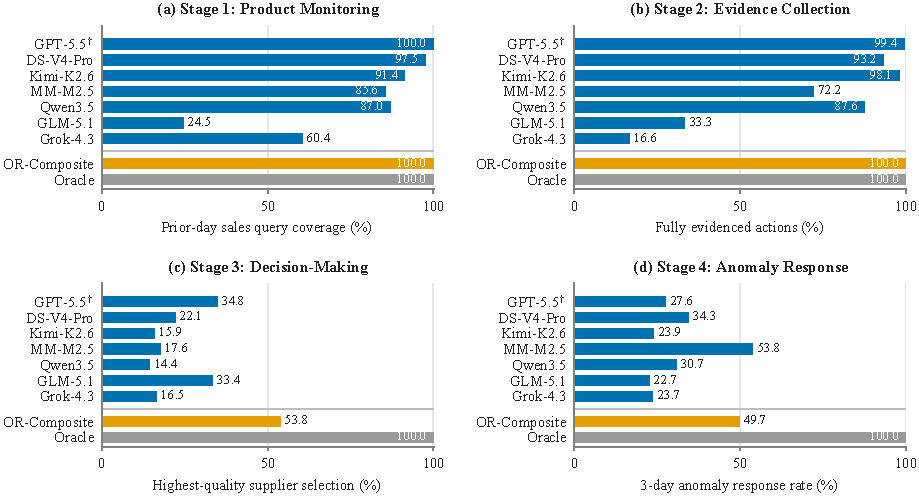
\includegraphics[width=\textwidth]{figures/four_stage_scores.pdf}
   \caption{Model-level outcome summary.
Results are reported as mean $\pm$ sample standard deviation
across three scaffolds, except GPT-5.5 (ReAct only).
LLM agents substantially underperform both references,
with the best LLM achieving only 30.1\% of OR-Composite's
final net worth.
Bold and underline indicate the best and second-best LLM results.
OR-Composite uses only agent-visible information
(Appendix~\ref{appendix:or_composite}),
while Oracle is a privileged reference
(Appendix~\ref{appendix:handcrafted_policy}).}
    \label{fig:four_stage_scores}
    \vspace{-2mm}
\end{figure*}

\paragraph{Long-horizon operational performance.}
Table~\ref{tab:aggregate_main_results} summarizes performance across ReAct, Reflection, and Plan-and-Act for the six models with complete scaffold coverage, reporting means and sample standard deviations across scaffolds rather than independent trials. GPT-5.5 is evaluated under ReAct only. No scaffold consistently dominates, with ReAct, Reflection, and Plan-and-Act achieving win counts of 2/2/2 for both final net worth and sales, and 3/1/2 for survival. Results for all 19 rollouts and the scaffold win counts are provided in Appendix~\ref{appendix:rollout_results}.

Results reveal substantial limitations in sustaining effective operations over long horizons. Mean survival ranges from 40.3 days (Grok-4.3) to 139.3 days (DeepSeek-V4-Pro), with none of the six fully evaluated models reaching the 180-day horizon on average. Only two of 19 rollouts complete all 180 days: DeepSeek-V4-Pro with Plan-and-Act and GPT-5.5 with ReAct. Moreover, completing the horizon does not guarantee strong business performance. The privileged Oracle achieves a final net worth of 124{,}491.15 and sales of 263{,}310 units, compared with 80{,}801.21 and 202{,}557 units for OR-Composite. DeepSeek-V4-Pro achieves the highest across-scaffold mean sales among fully evaluated models (110{,}980 units), while GPT-5.5 (ReAct), despite completing the full horizon, achieves only 24{,}350.98 in final net worth and 136{,}405 units in sales. These results reveal a substantial gap between sustained operation and effective long-horizon business performance.

\paragraph{Four-stage decision-making diagnosis.}
To examine where these performance gaps arise, we analyze agent trajectories across four stages: product monitoring, evidence collection, decision-making, and anomaly response (Section~\ref{sec:four_stage_setup}). Figure~\ref{fig:four_stage_scores} reports the corresponding diagnostic scores, with LLM results averaged over evaluated scaffolds. We additionally report pooled statistics across all 19 rollouts and individual-rollout ranges. These analyses are descriptive, with one rollout per model--scaffold configuration. Detailed breakdowns are provided in Appendix~\ref{appendix:stage_metrics}.

\paragraph{Four-stage decision-making diagnosis.}
To characterize the observed performance gaps, we analyze agent
trajectories across four stages: product monitoring, evidence collection,
decision-making, and anomaly response
(Section~\ref{sec:four_stage_setup}).
Figure~\ref{fig:four_stage_scores} summarizes the corresponding
diagnostic scores across models and reference policies.
A general pattern emerges: LLM agents perform relatively well
in product monitoring and evidence collection, but show substantially
weaker performance in decision-making and anomaly response.
We further examine these patterns using pooled statistics from
all 19 rollouts and individual-rollout results.
These analyses are descriptive, with one rollout per
model--scaffold configuration. Detailed results are provided
in Appendix~\ref{appendix:stage_metrics}.

\paragraph{Product Monitoring and evidence collection: effective information acquisition.}
As shown in Figure~\ref{fig:four_stage_scores}, most models
perform relatively well in the first two stages.
Across all LLM rollouts, 91.8\% of 31{,}527 sold
product--days receive a product-specific query on the following
day. Five of seven models achieve mean Stage~1 scores above
85\%, while GPT-5.5, DeepSeek-V4-Pro, and Kimi-K2.6 exceed
93\% in Stage~2. In contrast, GLM-5.1 and Grok-4.3 exhibit
substantially lower scores, particularly in evidence collection
(33.3\% and 16.6\%, respectively).
These results suggest that information acquisition is
relatively reliable among stronger agents, although
substantial variation remains across models.

\paragraph{Decision-making: shallow evidence-to-decision integration.}
Despite relatively strong evidence collection,
Figure~\ref{fig:four_stage_scores} reveals a pronounced
decline in supplier decision-making scores.
Across 5{,}172 order lines, LLM agents select the
highest-quality supplier in only 21.6\% of cases,
close to the 20\% random-choice baseline.
Model-level means range from 14.4\% to 34.8\%,
compared with 53.8\% for OR-Composite.
Although GLM-5.1 with Plan-and-Act achieves 56.0\%,
this result is based on only 50 orders.
As agents observe noisy quality signals and must balance
supplier quality against price, this metric does not
directly measure business decision optimality.
Nevertheless, considered alongside their weaker overall
business outcomes, these findings suggest
\textbf{shallow evidence-to-decision integration}:
agents struggle to translate acquired information
into economically effective decisions.

\paragraph{Anomaly response: inconsistent operational follow-up.}
Figure~\ref{fig:four_stage_scores} further shows limited
responsiveness to operational anomalies.
Among 2{,}374 eligible stockout and expiration events,
only 33.7\% are followed by an order or price adjustment
within three days, with response rates of 35.0\% for
stockouts and 22.8\% for expirations.
An additional 86 events are right-censored.
Model-level response rates range from 22.7\% to 53.8\%,
with no individual rollout exceeding 57.0\%.
Importantly, response frequency does not necessarily
reflect corrective effectiveness: OR-Composite achieves
a lower response rate than MiniMax-M2.5
(49.7\% vs. 53.8\%), yet substantially higher final
net worth (80{,}801.21 vs. 602.42).
Stage~4 therefore measures response coverage rather than
corrective effectiveness, revealing
\textbf{inconsistent operational follow-up}
among LLM agents.


\paragraph{Summary.}
Together, the outcome and trajectory analyses highlight persistent
challenges in long-horizon retail operations. Despite relatively
strong performance in product monitoring and evidence collection,
LLM agents exhibit near-chance supplier-quality selection, while
approximately two-thirds of eligible operational anomalies receive
no corresponding action within three days. These findings reveal
two recurring failure patterns:
\textbf{shallow evidence-to-decision integration} and
\textbf{limited responsiveness to salient operational anomalies},
which may partly explain the poor long-horizon performance
observed in some agents.